\section{Additional results}\label{app:additional}

\begin{table}[H]
\centering\small
\fittable{\tabdir/vol_validation_design.tex}
\caption{Design selection on the validation period 2010--2011 (training labels known before December 2009;
11\,115 market-days). ``vs HAR-IV'': MSE reduction relative to HAR-IV. The last row is the design used in
the walk-forward.}
\label{tab:design}
\end{table}

\begin{table}[H]
\centering\small
\fittable{\tabdir/vol_by_market.tex}
\caption{By market, 2012--2026: $R^2$ of HAR-IV and FuelGuard within each market, MSE reduction and DM
statistic of FuelGuard against HAR-IV (Newey--West, 21 lags; $<-1.96$: significantly better), and the best
single ML model.}
\end{table}

\begin{figure}[H]
\centering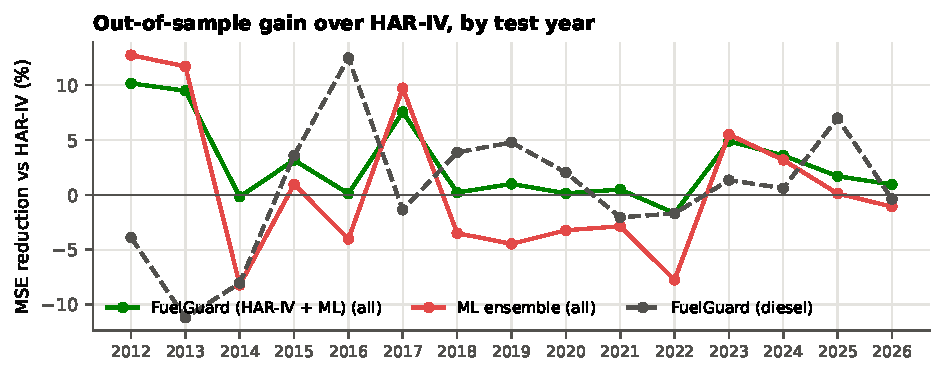
\includegraphics[width=0.95\textwidth]{v2_fig_by_year.pdf}
\caption{MSE reduction against HAR-IV by test year.}
\end{figure}

\begin{table}[H]
\centering\small
\fittable{\tabdir/vol_backtest.tex}
\caption{Diesel hedging backtest, 178 monthly decisions 2012--2026, hedge cost 1\%. Mean, St.dev, CVaR95
and Worst refer to the overrun of the monthly cost over the lockable price; EUR figures for 25\,000
litres a month.}
\label{tab:bt}
\end{table}

\begin{table}[H]
\centering\small
\fittable{\tabdir/vol_var_coverage.tex}
\caption{95\% worst-case bound: breaches over 178 monthly decisions (5\% expected), Kupiec test, average
bound, and breach rate over all daily decisions (overlapping windows).}
\end{table}

\begin{table}[H]
\centering\small
\fittable{\tabdir/vol_hyperparameters.tex}
\caption{Most frequent hyper-parameters chosen by purged cross-validation across the 15 training windows.}
\end{table}
